\documentclass[journal]{IEEEtran}
%
\usepackage{instructivo}  
\graphicspath{{./}{./fig/}}

\usepackage{circuitikz}
\usepackage{float}
\usepackage{graphicx}
\usepackage[skip=5pt]{caption}
\usepackage{flafter}
\usepackage{needspace}
\usepackage{csquotes}



\hyphenation{op-tical net-works semi-conduc-tor}

\renewcommand\IEEEkeywordsname{Palabras clave}

\begin{document}
\title{Topologías de amplificadores de fuente común y de drenador común con JFETs}


\author{Juan~P.~Elizondo~Espinoza,~\IEEEmembership{Estudiante,~TEC}
        y~Matías~A.~Camacho~Abarca,~\IEEEmembership{Estudiante,~TEC.}
}


\markboth{TEC.~EL-3215 Laboratorio de Electrónica Analógica, IS~2025}%
{EL3215 Laboratorio de Electrónica Analógica}


\maketitle


\begin{abstract}
El objetivo del experimento fue construir circuitos recortadores para entender el comportamiento de la onda de salida
teniendo en cuenta distintos casos de polarización. Se logró comprobar el comportamiento teórico esperado de los circuitos a través de un análisis visual.
\end{abstract}

\begin{IEEEkeywords}
Diodo, tensión, corriente, junta, ruptura.
\end{IEEEkeywords}


%%%%%%%%%%%%%%%%%%%%%%%%%%%%%%%%%%%%%%%%%%%%%%%%%%%%%%%%%%%%%%%%%%%%%%%%%%%%%%%%%%%%%%%%%%%%%%
%%%%%%%%%%%%%%%%%%%%%%%%%%%%%%%%%%%%%%%%%%%%%%%%%%%%%%%%%%%%%%%%%%%%%%%%%%%%%%%%%%%%%%%%%%%%%%
\section{Introducción}

\IEEEPARstart{U}n diodo es un componente electrónico de dos terminales que permite el flujo de corriente en una dirección y lo bloquea en la otra. Está formado por la unión de dos materiales semiconductores con diferente tipo de dopaje: tipo p y tipo n.

El material tipo p se forma al dopar semiconductores como el silicio o el germanio con impurezas de tres electrones de valencia, como el boro, lo que genera una abundancia de huecos (cargas positivas). Por otro lado, el material tipo n se obtiene al agregar impurezas con cinco electrones de valencia, como el fósforo o el arsénico, lo que introduce electrones libres en la estructura.

Al unir ambos materiales en un solo dispositivo, se forma una unión pn, la base del funcionamiento del diodo. Idealmente, los huecos pueden moverse desde la región p hacia la región n, siguiendo la dirección de la corriente convencional. Sin embargo, si se intenta conducir corriente en la dirección opuesta (de n a p), la unión pn presenta una barrera que impide el flujo, actuando como un interruptor unidireccional.

Estas propiedades aplican para diodos ideales, ya que en la realidad los diodos tienen un rango de tensión necesario para que la
corriente fluya significativamente en polarización directa (corriente convencional de p a n). Los diodos incluso tienen corriente en polarización inversa (corriente convencional de n a p), aunque esta suele ser despreciable. Sin embargo, para efectos de análisis, se pueden 
generalizar muchas de estas propiedades.

Uno de los usos más particulares de los diodos es en circuitos recortadores. Estos se aprovechan del funcionamiento del diodo como una fuente de tensión en polarización directa
y como un nodo abierto en inversa. En estas aplicaciones, se elimina partes de la señal de entrada por encima o por debajo de cierto nivel de voltaje. Existen dos configuraciones principales: en serie y en paralelo.  

En los recortadores en paralelo, el diodo se coloca en paralelo con la carga y conduce solo cuando la señal supera un voltaje específico. Si el diodo está sin polarización externa, su umbral de conducción es aproximadamente 0 V en el modelo ideal.   

Estos circuitos son útiles para limitar amplitudes y proteger componentes sensibles frente a sobrevoltajes. En el modelo ideal, el diodo cambia instantáneamente entre conducción y no conducción, lo que permite una representación simplificada del comportamiento del circuito. \cite{Boylestad}


%%%%%%%%%%%%%%%%%%%%%%%%%%%%%%%%%%%%%%%%%%%%%%%%%%%%%%%%%%%%%%%%%%%%%%%%%%%%%%%%%%%%%%%%%%%%%%
%%%%%%%%%%%%%%%%%%%%%%%%%%%%%%%%%%%%%%%%%%%%%%%%%%%%%%%%%%%%%%%%%%%%%%%%%%%%%%%%%%%%%%%%%%%%%%
\section{Circuitos recortadores con Diodos}
Como una forma de entender el funcionamiento de estos dispositivos (los Diodos), se pueden diseñar circuitos que tengan amplias aplicaciones prácticas en la vida cotidiana,
dentro de estos están los circuitos recortadores, en donde los diodos juegan un papel muy importante y es posible establecer diferentes configuraciones según se requiera. 


\subsection{Circuitos de Medición}

El circuito de la Fig. \ref{fig:recortador_sinDiodo} se utiliza para ver el comportamiento de la señal de salida (modificada por medio de un divisor de tensión), respecto a la señal de entrada Vs.
\begin{figure}[H]
        \centering
        \begin{circuitikz}
                % Fuente de señal CA
                \draw (0,0) 
                   to[sV] (0,2.5) % Fuente de CA
                   node[left=0.7cm, yshift=-0.7cm] {$V_s$}
                   node[left=0.5cm, yshift=-1.2cm] {$6\,V_{pp}$}
                   node[left=0.4cm, yshift=-1.7cm] {$1\,kHz$};
                \draw (0,2.5) to [short] (2.5,2.5);

                % Resistencia en paralelo a la fuente
                \draw (2.5,2.5) to [R,l_=$R_1$, a^={10 k$\Omega$}] (2.5,0);

                % Resistencias en serie
                \draw (2.5,2.5) to [R, l^=$R_2$, a={1 k$\Omega$}] (5,2.5);
                \draw (5,2.5) to [R,l_=$R_L$, a^={100 k$\Omega$}] (5,0);

                \draw (5,0) to [short] (0,0);
        \end{circuitikz}
        \caption{Circuito recortador sin Diodo}
        \label{fig:recortador_sinDiodo}
\end{figure}

Luego, se modifica el circuito anterior al agregarle un diodo, de manera que ahora es un circuito recortador que utiliza un elemento activo. Según se muestra en la Fig. \ref{fig:recortador_conDiodo}.
Considere que los valores de las resistencias se mantienen iguales a los del circuito en la Fig. \ref{fig:recortador_sinDiodo}.
\begin{figure}[H]
        \centering
        \begin{circuitikz}
                % Fuente de señal CA
                \draw (0,0) 
                   to[sV] (0,2.5) % Fuente de CA
                   node[left=0.7cm, yshift=-0.7cm] {$V_s$}
                   node[left=0.5cm, yshift=-1.2cm] {$6\,V_{pp}$}
                   node[left=0.4cm, yshift=-1.7cm] {$1\,kHz$};
                \draw (0,2.5) to [short] (2,2.5);

                % Resistencia
                \draw (2,2.5) to [R,l_=$R_1$] (2,0);
                \draw (2,2.5) to [R, l^=$R_2$] (4.5,2.5);
                \draw (4.5,2.5) to [short] (6.5,2.5);
                \draw (6.5,2.5) to [R,l_=$R_L$] (6.5,0);
                \draw (6.5,0) to [short] (0,0);


                % Diodo IN914
                %\draw (4.5,2.5) to [D, l=$D_1$, fill=black] (4.5,0);
                \draw (4.5,2.5)
                   to[D, fill=black] (4.5,0)
                   node[left=0.3cm, yshift=1.3cm] {$D_1$}
                   node[left=0.3cm, yshift=0.9cm] {1N914};

        \end{circuitikz}
        \caption{Circuito recortador con Diodo}
        \label{fig:recortador_conDiodo}
\end{figure}

Como tercera modificación, se le agrega una fuente en CD en serie con el diodo al circuito según la Fig. \ref{fig:recortador_conAjuste}, que agrega un ajuste a la tensión vista por la carga. 
\begin{figure}[H]
        \centering
        \begin{circuitikz}
                % Fuente de señal CA
                \draw (0,0) 
                to[sV] (0,3) % Fuente de CA
                   node[left=0.7cm, yshift=-1cm] {$V_s$}
                   node[left=0.5cm, yshift=-1.5cm] {$6\,V_{pp}$}
                   node[left=0.4cm, yshift=-2cm] {$1\,kHz$};
                \draw (0,3) to [short] (2,3);

                % Resistencia
                \draw (2,3) to [R,l_=$R_1$] (2,0);
                \draw (2,3) to [R, l^=$R_2$] (4.5,3);
                \draw (4.5,3) to [short] (6.5,3);
                \draw (6.5,3) to [R,l_=$R_L$] (6.5,0);
                \draw (6.5,0) to [short] (0,0);

                % Diodo IN914
                %\draw (4.5,3) to [D, l=$D_1$, fill=black] (4.5,1.25);
                \draw (4.5,3)
                   to[D, fill=black] (4.5,1.25)
                   node[left=0.3cm, yshift=1.0cm] {$D_1$}
                   node[left=0.3cm, yshift=0.6cm] {1N914};

                % Fuente de CD
                \draw (4.5,1.25) to [battery, l_=$V_{CD}$] (4.5,0);
        \end{circuitikz}
        \caption{Circuito recortador con Diodo con ajuste}
        \label{fig:recortador_conAjuste}
\end{figure}
\vspace{-0.8cm}

\needspace{5\baselineskip}
\subsection{Simulaciones}
Acá se muestran y describen los resultados teóricos esperados por medio de simulaciones, para este caso corresponden a gráficas de señales en su mayoría. 
Del circuito mostrado en la FIg. \ref{fig:recortador_sinDiodo} se obtienen las siguientes señales simuladas.

\begin{figure}[H]
        \centering
        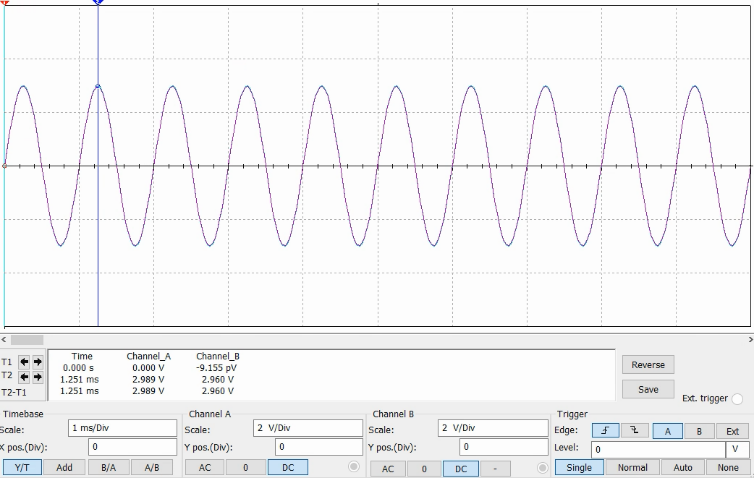
\includegraphics[width=2.7in]{SignalSimulated_01.png}
        \caption{Señales de salida y entrada del circuito recortador sin Diodo (simulado).}
        \label{fig:SignalSimulated_01}
\end{figure}

Ambas señales en la Fig. \ref{fig:SignalSimulated_01} se ven prácticamente iguales, ya que el valor de $R_1$ respecto a $R_L$, es muy pequeño. Por otro lado, en la Fig. \ref{fig:SignalSimulated_02} se muestra la simulación del circuito de la Fig. \ref{fig:recortador_conDiodo}.
\begin{figure}[H]
        \centering
        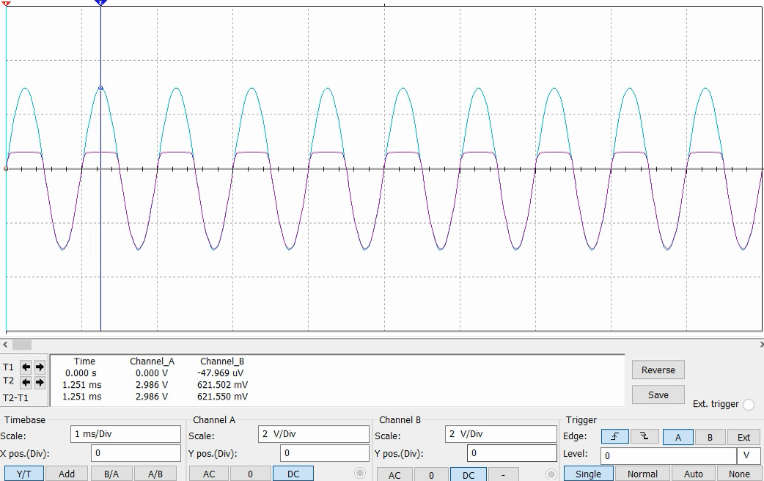
\includegraphics[width=2.7in]{SignalSimulated_02.png}
        \caption{Señales de salida y entrada del circuito recortador con Diodo (simulado).}
        \label{fig:SignalSimulated_02}
\end{figure}

En la Fig. \ref{fig:SignalSimulated_02} existen diferencias más notorias entre las señales de entrada y salida. Ahora, para el mismo circuito de la Fig. \ref{fig:recortador_conDiodo}, se muestra la señal de tensión presente en la resistencia $R_2$.

\begin{figure}[htbp]
        \centering
        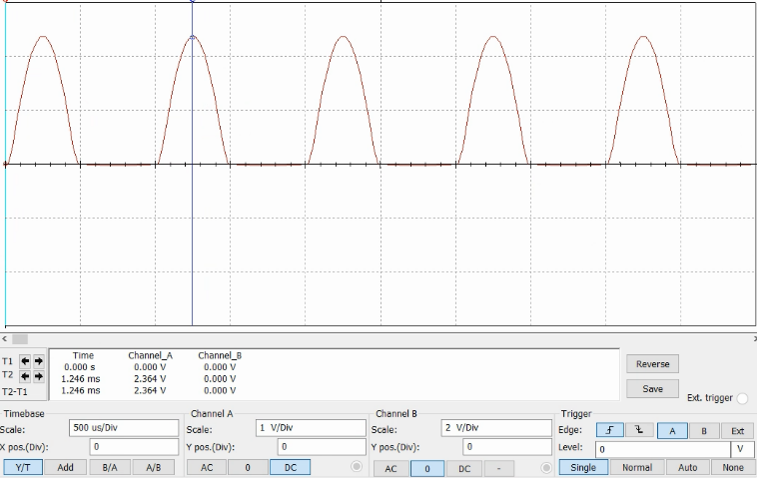
\includegraphics[width=2.7in]{SignalSimulated_03.png}
        \caption{Señal de tensión en la resistencia $R_2$ (simulado).}
        \label{fig:SignalSimulated_03}
\end{figure}

Seguidamente, al cambiar la resistencia de carga $R_L$ por uno cuyo valor sea de $10~\textnormal{k}\Omega$, se tienen las siguientes señales de entrada y salida para el circuito mostrado en la Fig. \ref{fig:recortador_conDiodo}
\begin{figure}[htbp]
        \centering
        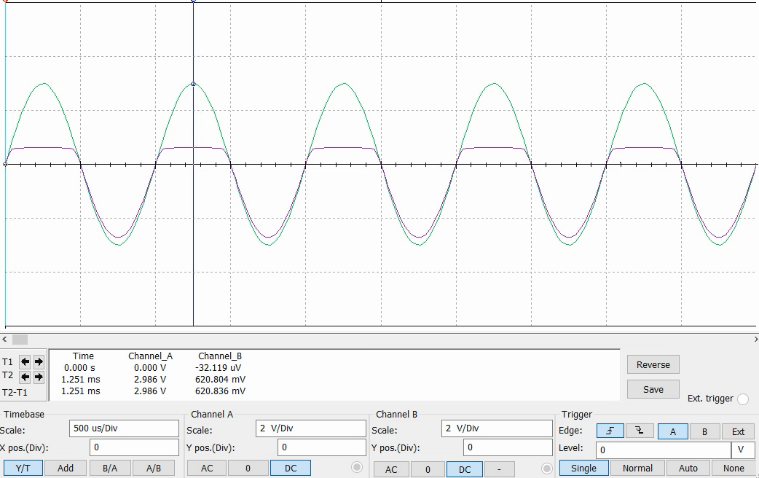
\includegraphics[width=2.7in]{SignalSimulated_04.png}
        \caption{Señales de salida y entrada del circuito recortador con Diodo, con $R_L=10~\textnormal{k}\Omega$ (simulado).}
        \label{fig:SignalSimulated_04}
\end{figure}

A continuación, restableciendo la resistencia $R_L$ a su valor original de $100~\textnormal{k}\Omega$, se modifica de manera que resulta en el circuito de la Fig. \ref{fig:recortador_conAjuste}.
Se hacen variaciones en la fuente de CD, desde los $0~\textnormal{V}$ hasta los $2~\textnormal{V}$, con pasos de $500~\textnormal{mV}$. Obteniendo las siguientes señales.

\begin{figure}[H]
        \centering
        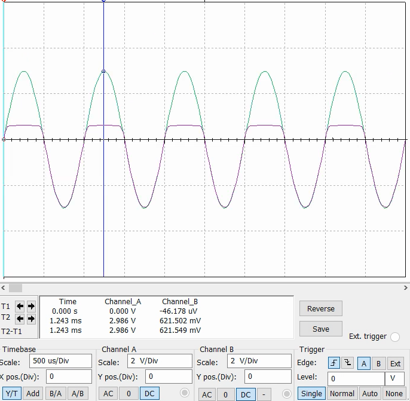
\includegraphics[width=2.7in]{SignalSimulated_05.png}
        \caption{Circuito recortador con fuente de CD en $0~\textnormal{V}$ (simulado).}
        \label{fig:SignalSimulated_05}
\end{figure}
\vspace{-0.5cm}
\begin{figure}[H]
        \centering
        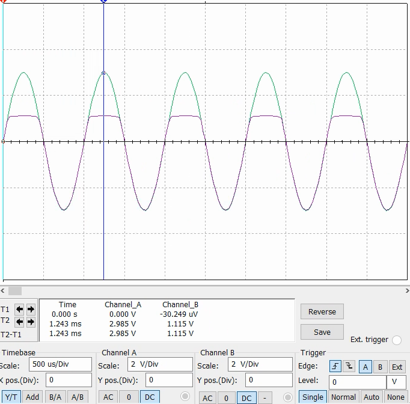
\includegraphics[width=2.7in]{SignalSimulated_06.png}
        \caption{Circuito recortador con fuente de CD en $500~\textnormal{mV}$ (simulado).}
        \label{fig:SignalSimulated_06}
\end{figure}
\begin{figure}[H]
        \centering
        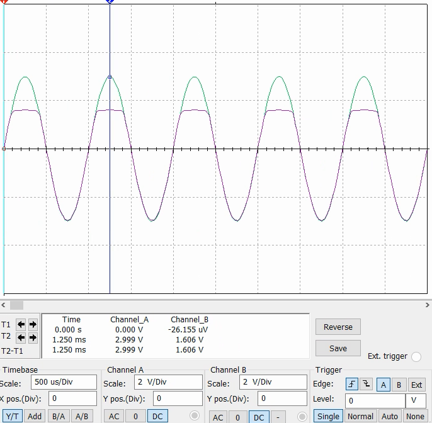
\includegraphics[width=2.7in]{SignalSimulated_07.png}
        \caption{Circuito recortador con fuente de CD en $1~\textnormal{V}$ (simulado).}
        \label{fig:SignalSimulated_07}
\end{figure}
\begin{figure}[H]
        \centering
        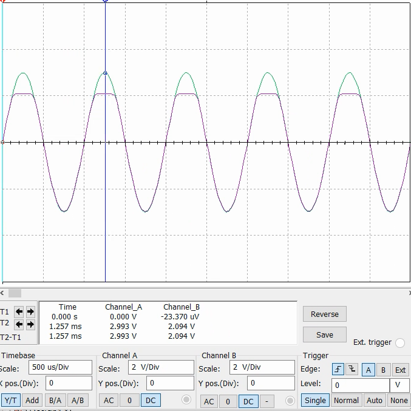
\includegraphics[width=2.7in]{SignalSimulated_08.png}
        \caption{Circuito recortador con fuente de CD en $1.5~\textnormal{V}$ (simulado).}
        \label{fig:SignalSimulated_08}
\end{figure}

\begin{figure}[H]
        \centering
        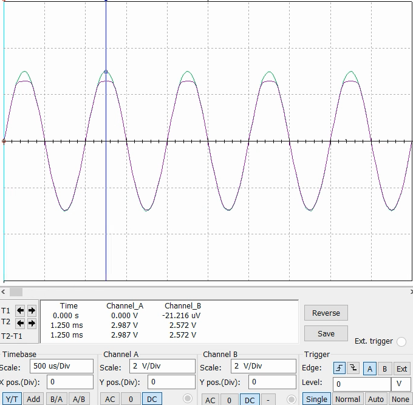
\includegraphics[width=2.7in]{SignalSimulated_09.png}
        \caption{Circuito recortador con fuente de CD en $2~\textnormal{V}$ (simulado).}
        \label{fig:SignalSimulated_09}
\end{figure}


Como se observa a los largo de todas las figuras presentadas anteriormente, el aumentar la magnitud de la fuente de CD
genera que la señal de tensión vista desde la resistencia de carga vaya aumentando poco a poco, de cierta forma acercándose 
a la señal de entrada. Seguidamente, se procede a invertir la conexión del diodo 1N914 para repetir el proceso de aumentar 
la fuente de CD desde los $0~\textnormal{V}$ hasta los $2~\textnormal{V}$, con pasos de $500~\textnormal{mV}$.
\begin{figure}[H]
        \centering
        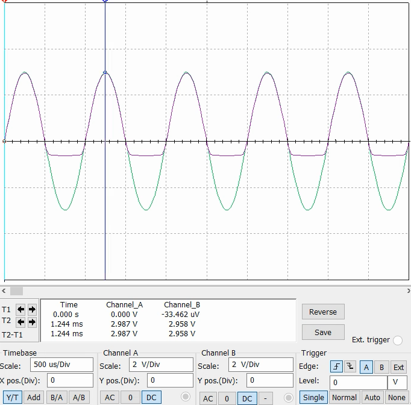
\includegraphics[width=2.7in]{SignalSimulated_10.png}
        \caption{Circuito recortador con Diodo invertido y fuente de CD en $0~\textnormal{V}$ (simulado).}
        \label{fig:SignalSimulated_10}
\end{figure}
\vspace{-0.6cm}
\begin{figure}[H]
        \centering
        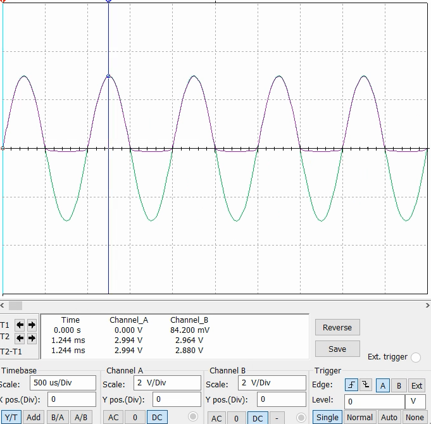
\includegraphics[width=2.7in]{SignalSimulated_11.png}
        \caption{Circuito recortador con Diodo invertido y fuente de CD en $500~\textnormal{mV}$ (simulado).}
        \label{fig:SignalSimulated_11}
\end{figure}
\begin{figure}[H]
        \centering
        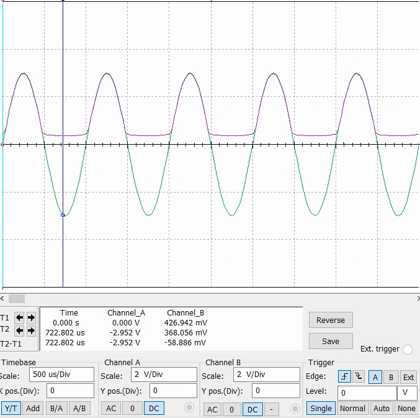
\includegraphics[width=2.7in]{SignalSimulated_12.png}
        \caption{Circuito recortador con Diodo invertido y fuente de CD en $1~\textnormal{V}$ (simulado).}
        \label{fig:SignalSimulated_12}
\end{figure}
\begin{figure}[H]
        \centering
        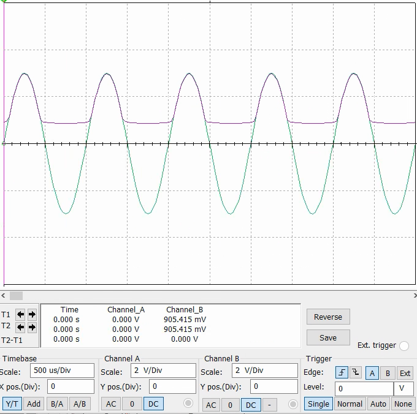
\includegraphics[width=2.7in]{SignalSimulated_13.png}
        \caption{Circuito recortador con Diodo invertido y fuente de CD en $1.5~\textnormal{V}$ (simulado).}
        \label{fig:SignalSimulated_13}
\end{figure}
\begin{figure}[H]
        \centering
        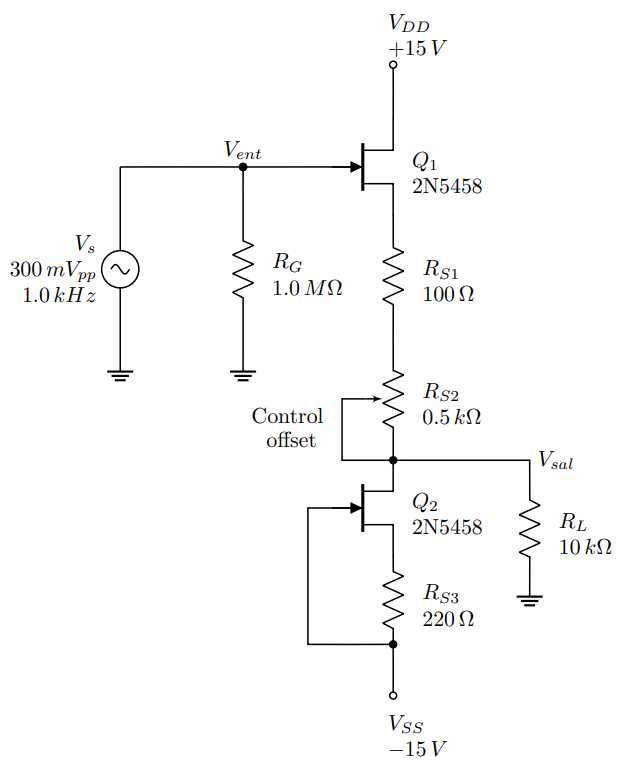
\includegraphics[width=2.7in]{CIRC2_2.png}
        \caption{Circuito recortador con Diodo invertido y fuente de CD en $2~\textnormal{V}$ (simulado).}
        \label{fig:SignalSimulated_14}
\end{figure}

En el escenario anterior se observa el mismo efecto al aumentar el valor de la fuente en CD; sin embargo, considerando
que la polaridad del diodo se invirtió, la señal de salida se ve afectada de manera contraria a la presentada en el caso anterior.
De forma que ahora la señal vista por la carga, disminuye cada vez menos su magnitud con cada periodo completado.

Finalmente, manteniendo el diodo invertido, se invierte además la polaridad de la fuente en CD, tal que ahora será como que si la fuente
entregara valores de tensión negativos; de igual forma, se repite el proceso iterativo pero ahora desde los $0~\textnormal{V}$ hasta los $-2~\textnormal{V}$, con pasos de $500~\textnormal{mV}$.
\begin{figure}[H]
        \centering
        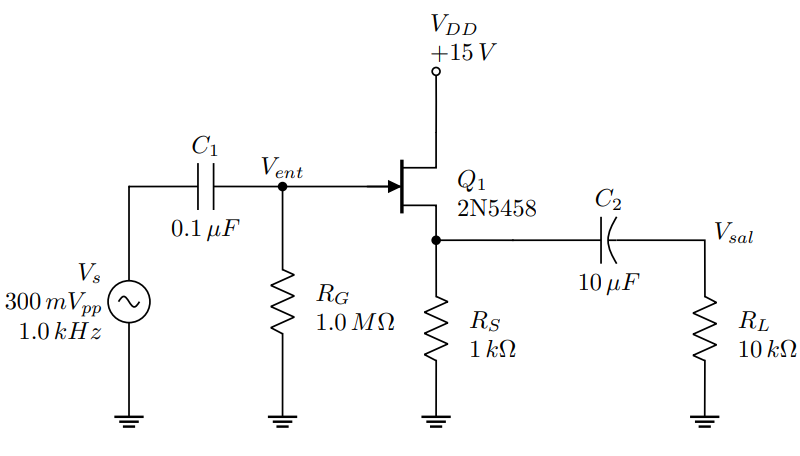
\includegraphics[width=2.7in]{CIRC2.png}
        \caption{Circuito recortador con Diodo invertido y fuente de CD en $0~\textnormal{V}$ (simulado).}
        \label{fig:SignalSimulated_15}
\end{figure}
\vspace{-0.6cm}
\begin{figure}[H]
        \centering
        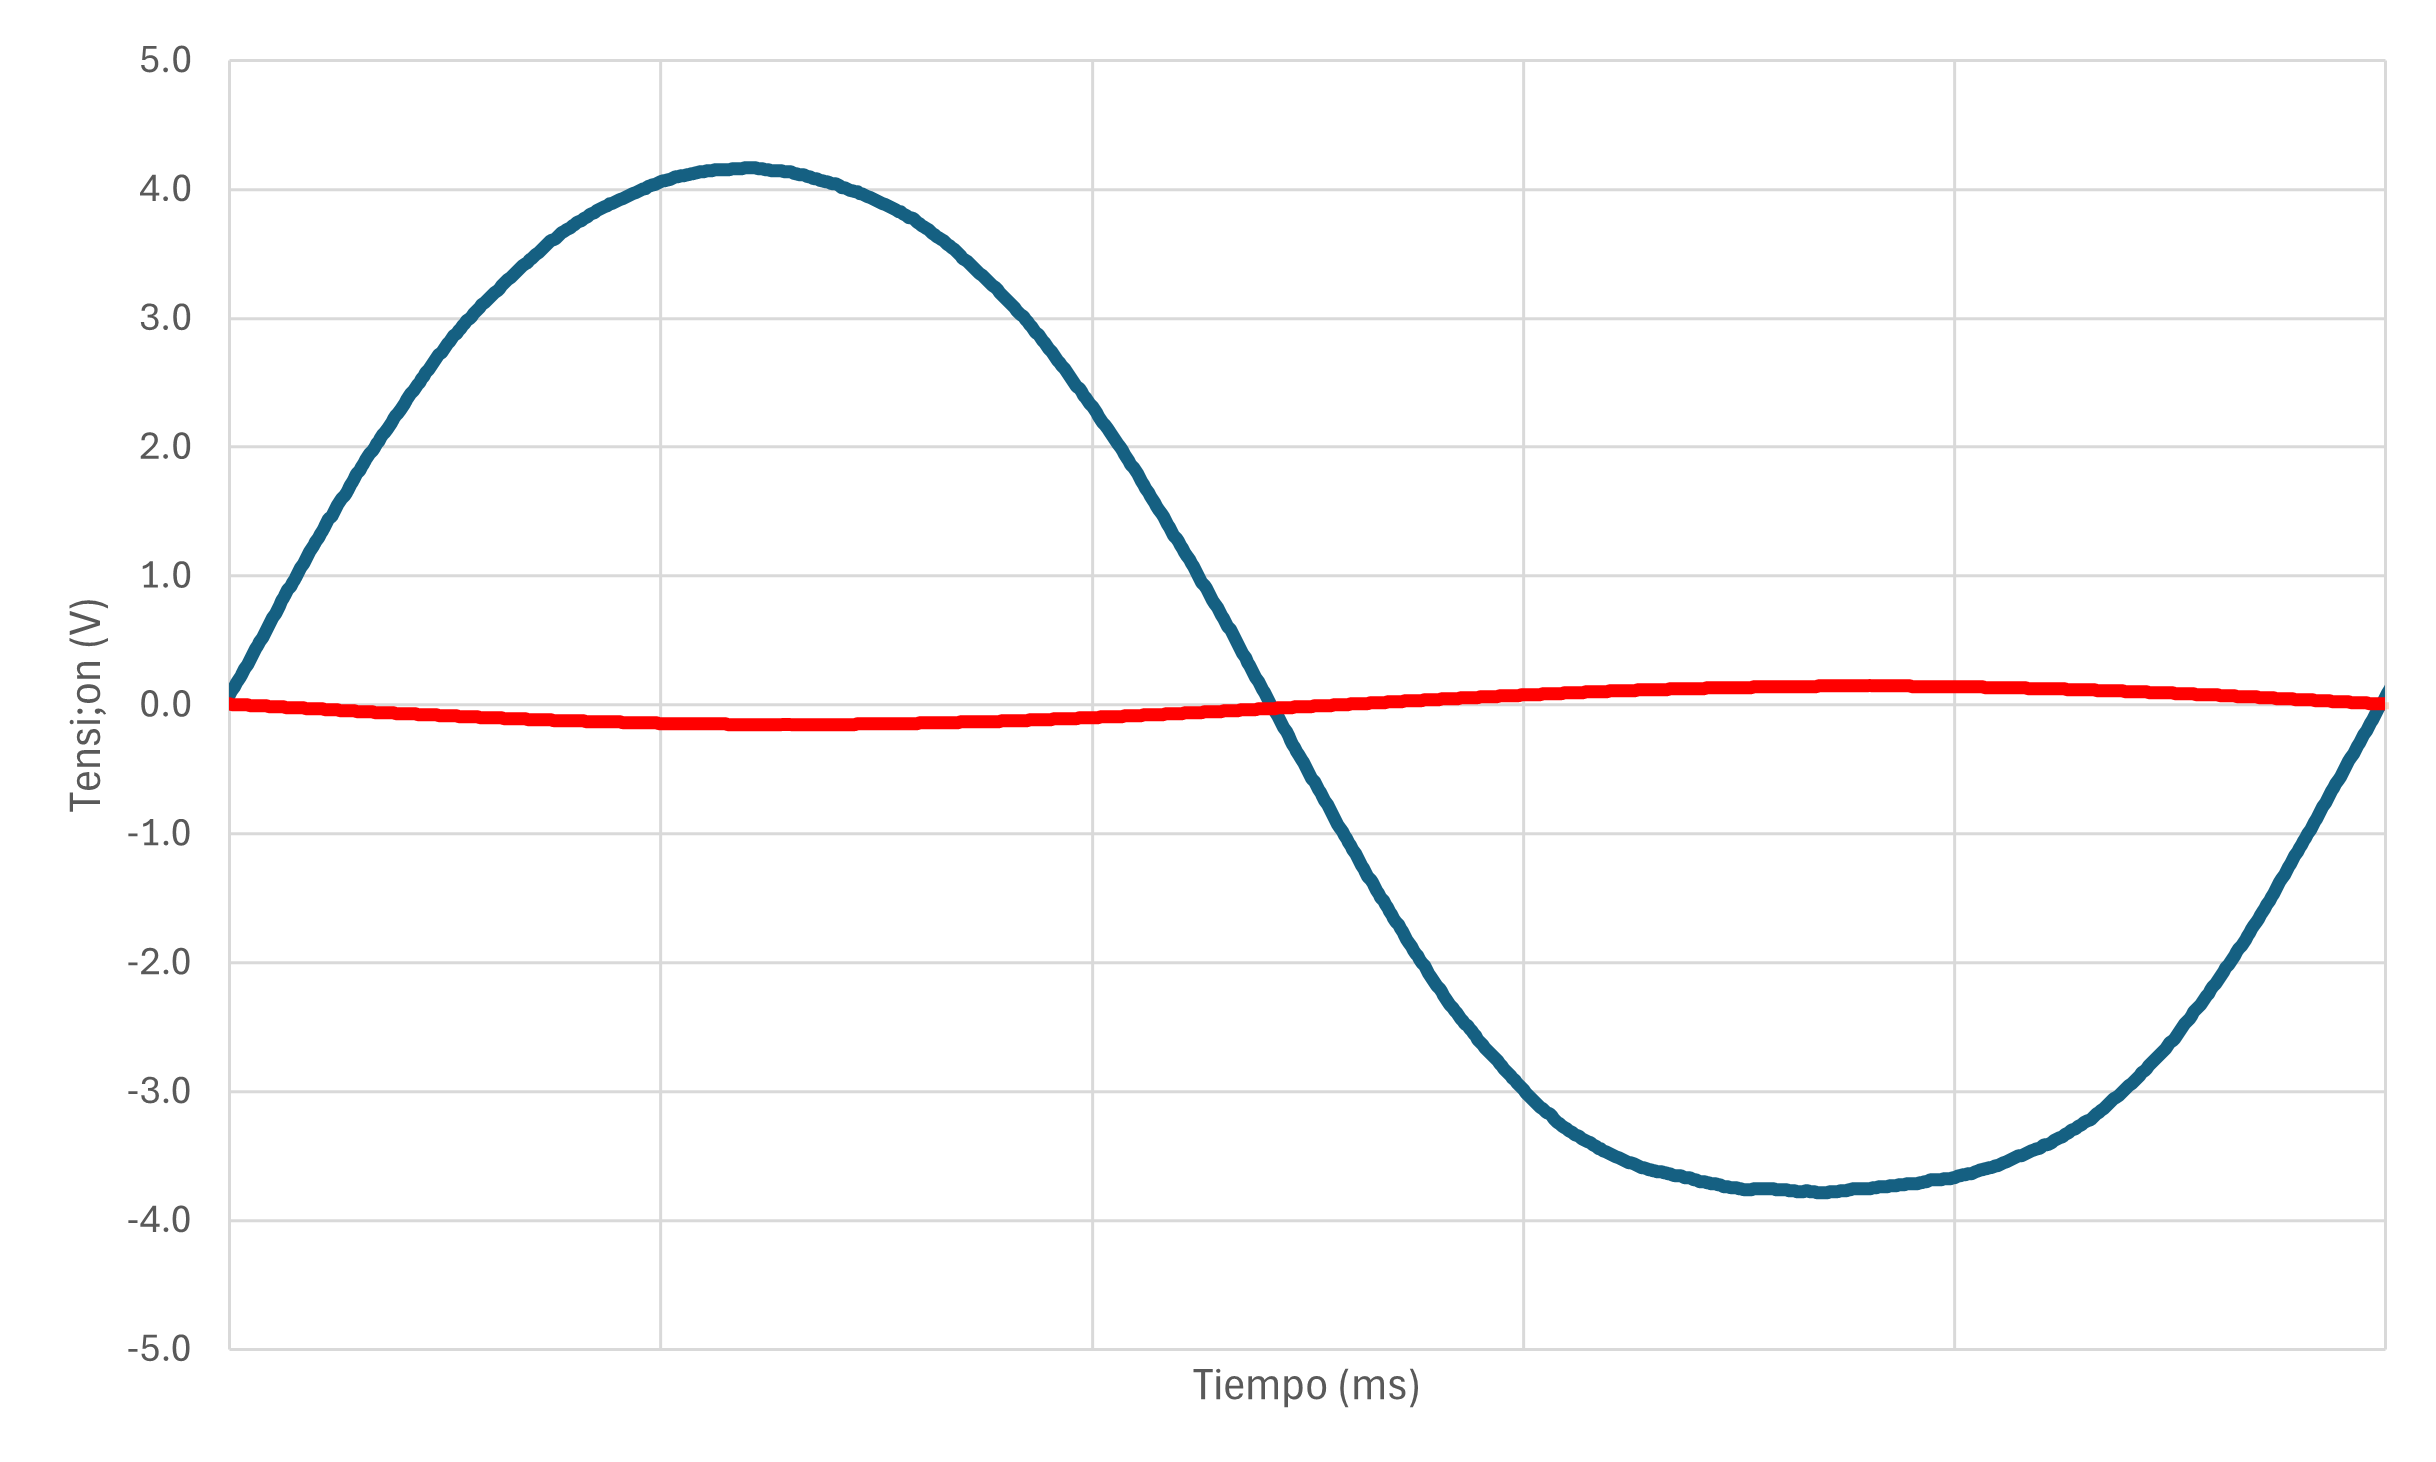
\includegraphics[width=3.3in]{C1111.png}
        \caption{Circuito recortador con Diodo invertido y fuente de CD en $-500~\textnormal{mV}$ (simulado).}
        \label{fig:SignalSimulated_16}
\end{figure}
\begin{figure}[H]
        \centering
        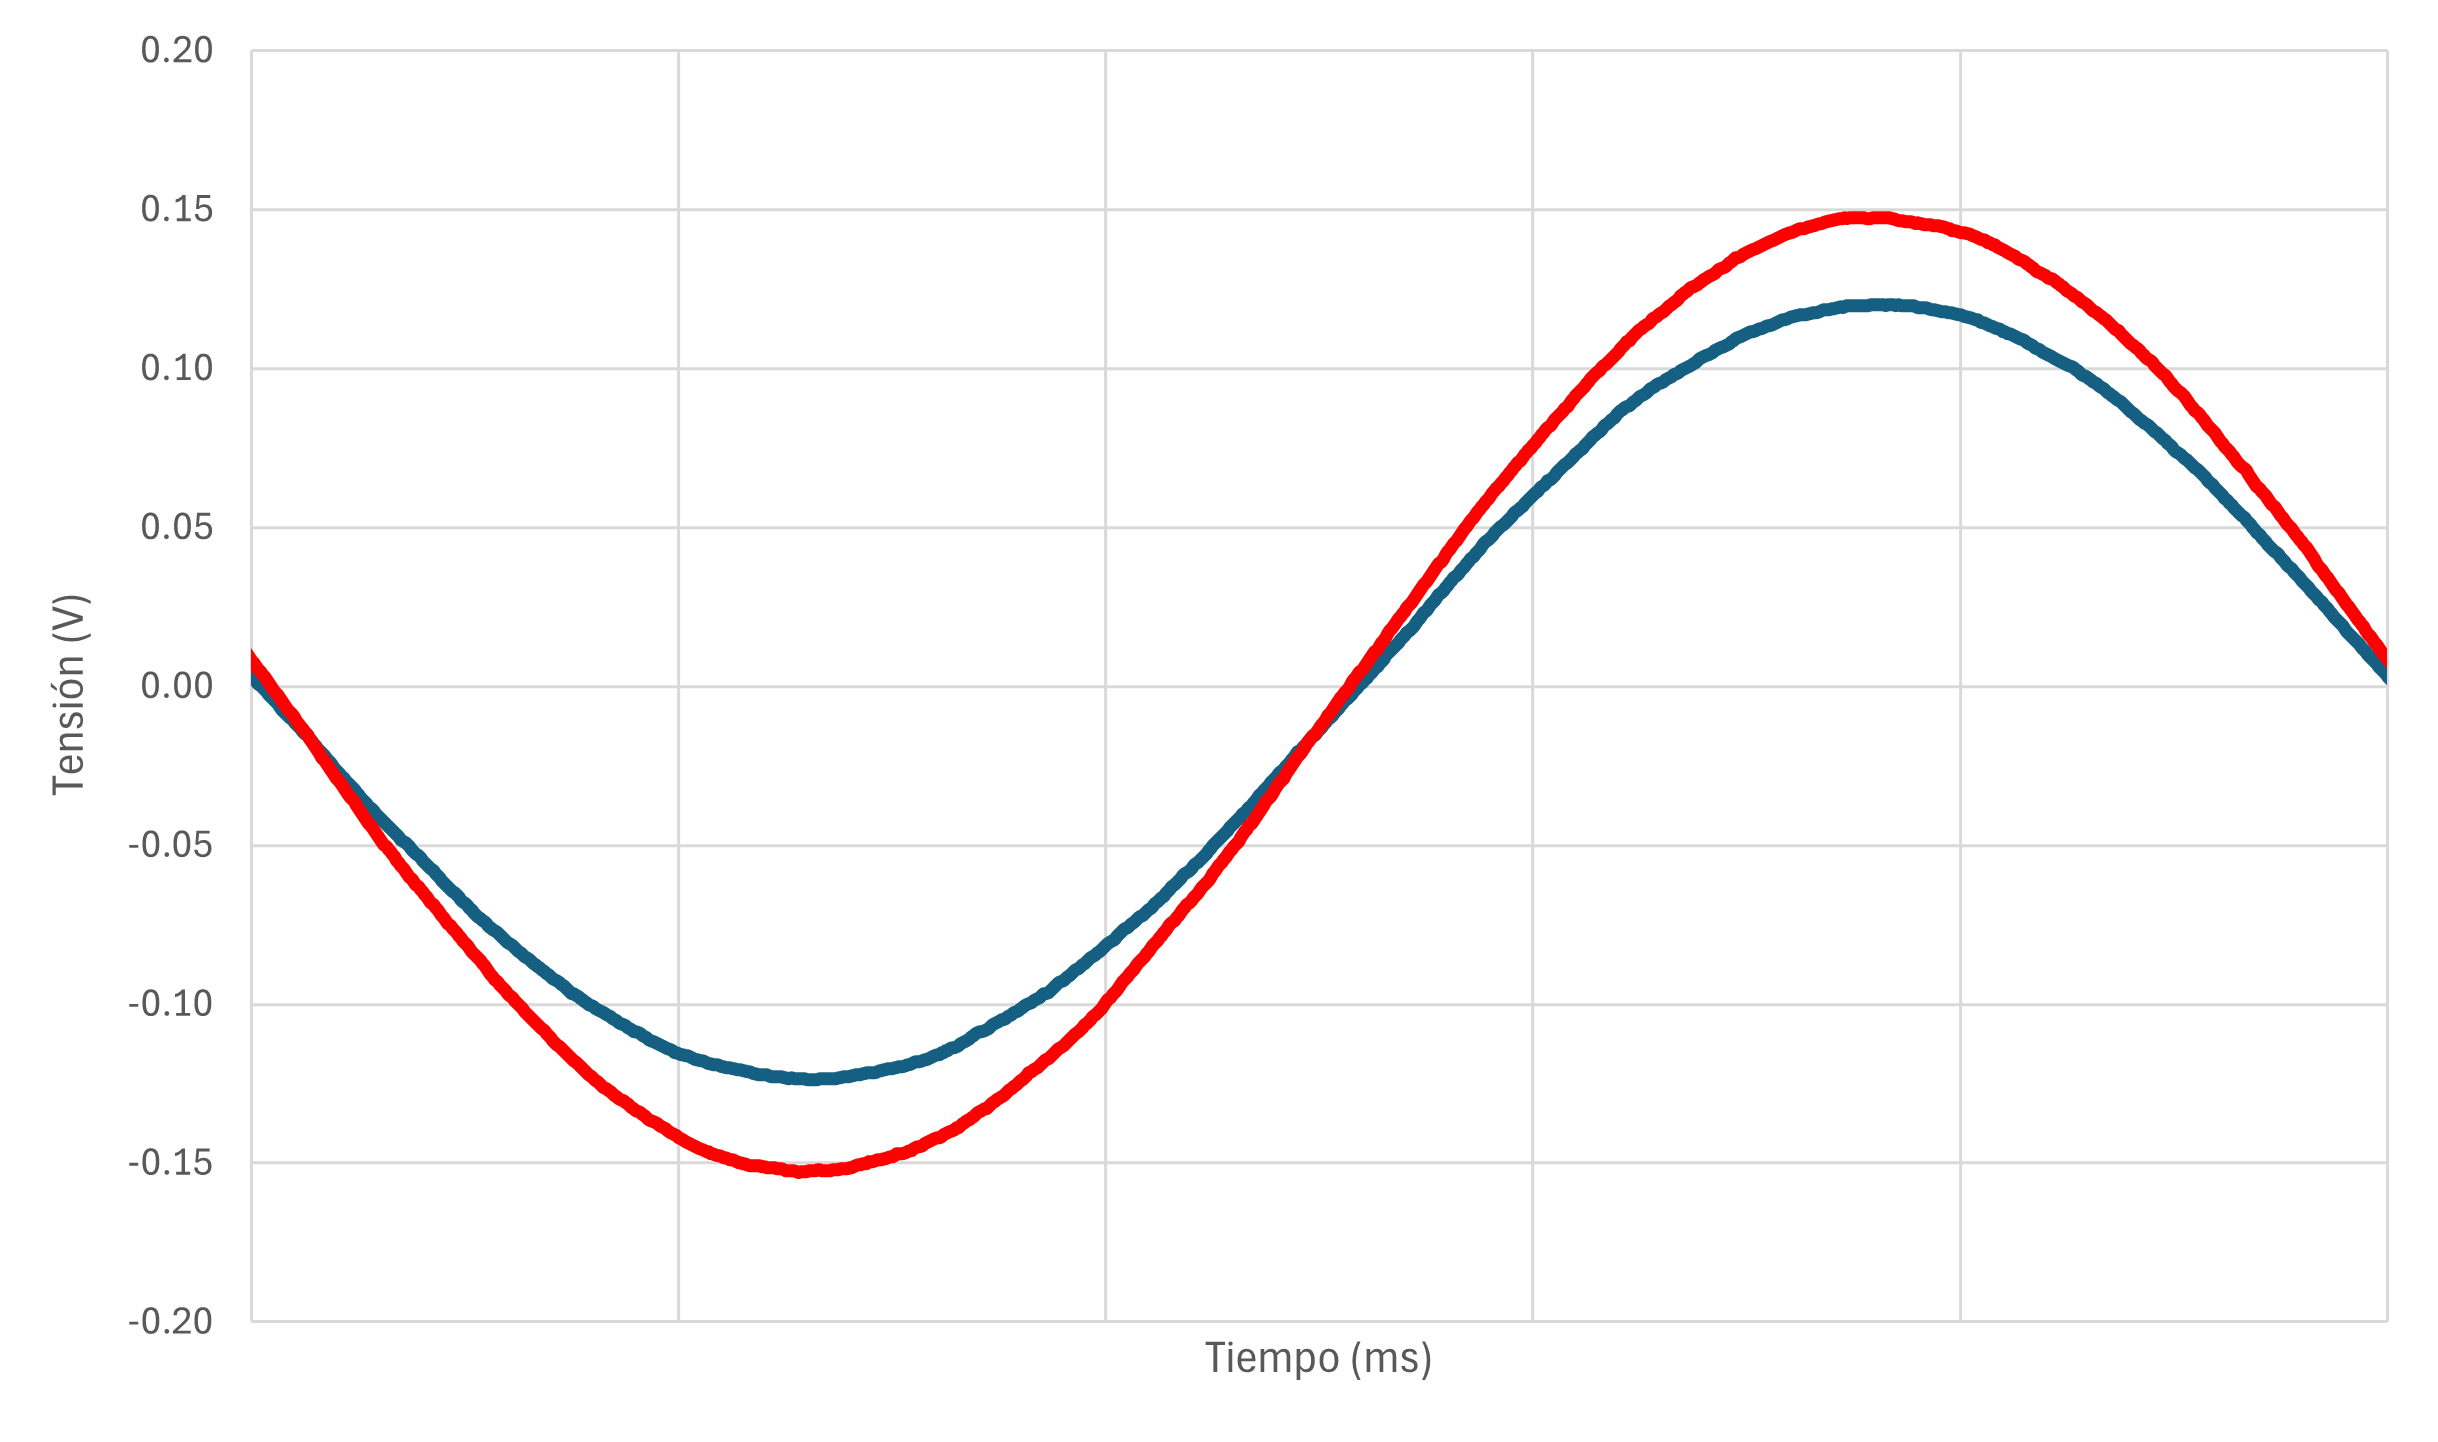
\includegraphics[width=3.3in]{C2222.png}
        \caption{Circuito recortador con Diodo invertido y fuente de CD en $-1~\textnormal{V}$ (simulado).}
        \label{fig:SignalSimulated_17}
\end{figure}
\begin{figure}[H]
        \centering
        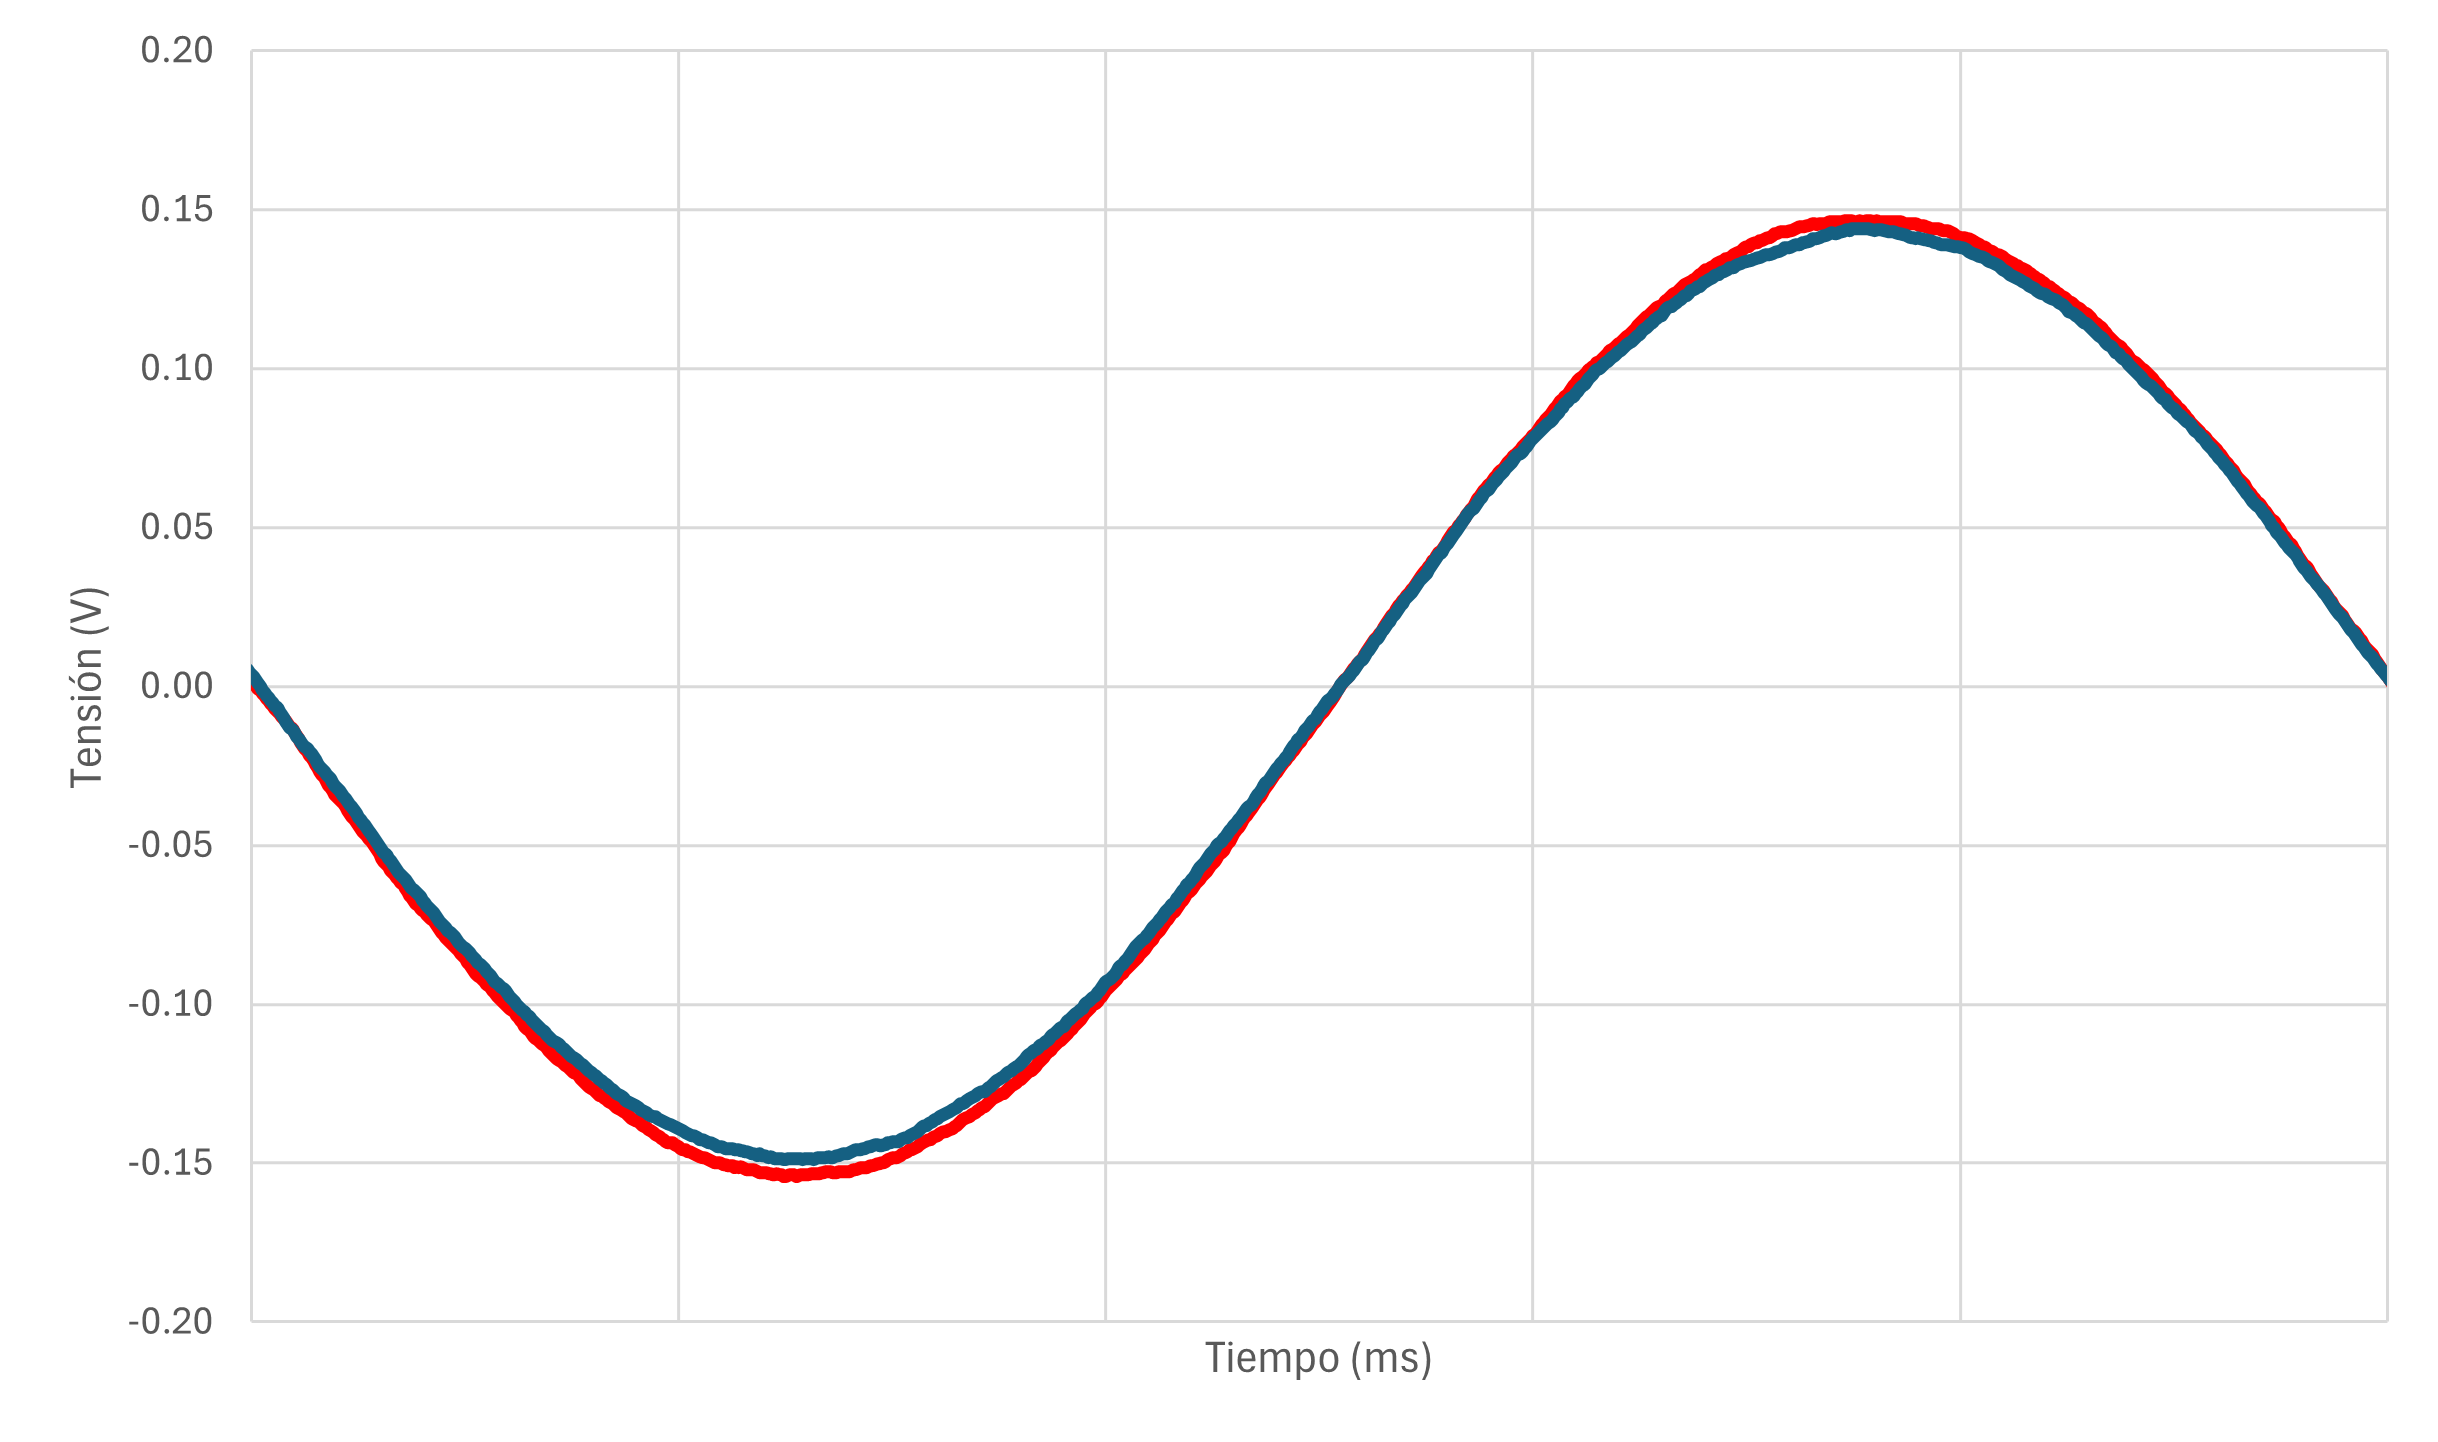
\includegraphics[width=3.3in]{2C2222.png}
        \caption{Circuito recortador con Diodo invertido y fuente de CD en $-1.5~\textnormal{V}$ (simulado).}
        \label{fig:SignalSimulated_18}
\end{figure}
\begin{figure}[H]
        \centering
        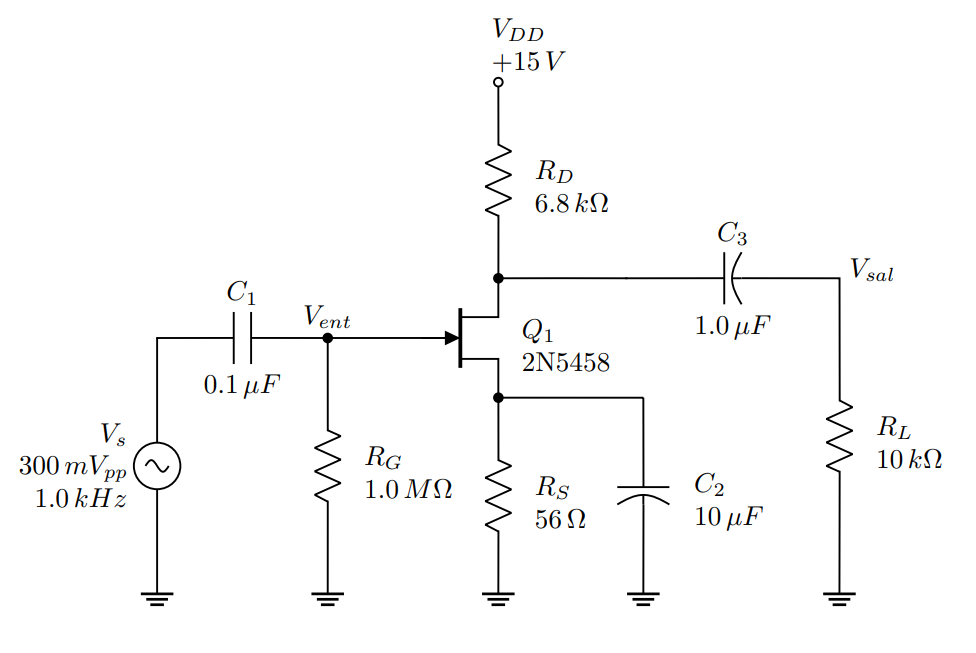
\includegraphics[width=2.7in]{Circ1.png}
        \caption{Circuito recortador con Diodo invertido y fuente de CD en $-2~\textnormal{V}$ (simulado).}
        \label{fig:SignalSimulated_19}
\end{figure}

En este último caso con el diodo y la fuente invertidos, la señal de salida (vista por la carga) varía de forma que con cada disminución en la fuente de CD, su forma 
se acerca cada vez más a la señal de entrada, pero de forma inversa que al inicio, lo cual tiene bastante sentido lógico. 


\subsection{Resultados Experimentales}

Seguidamente, se muestran los datos experimentales recopilados en la sesión de laboratorio con ayuda de los instrumentos disponibles y los cricuitos necesarios.
Es importante tener en consideración que existen algunas variaciones con las señales teóricas por alteraciones en los componentes utilizados para el laboratorio.

Primeramente, se muestran los valores reales de las resistencias utilizadas. 

\begin{table}[H]
        \centering
        \renewcommand{\arraystretch}{1.5}
        \caption{Valores de resistencia utilizados}
        \begin{tabular}{ m{2cm} m{2cm} m{2cm} }
            \hline
            Componente & Valor requerido ($\textnormal{k}\Omega$) & Valor medido ($\textnormal{k}\Omega$) \\ 
            \hline
            $R_1$ & $10$ & $9.929~40$ \\ 
            $R_2$ & $1$ & $0.995~31$ \\
            $R_L$ & $100$ & $99.619~9$ \\
            \hline
        \end{tabular}
        \label{tabla1}
    \end{table}
    

Se presentan las señales de entrada y salida para el circuito de la Fig. \ref{fig:recortador_sinDiodo}.
\begin{figure}[H]
        \centering
        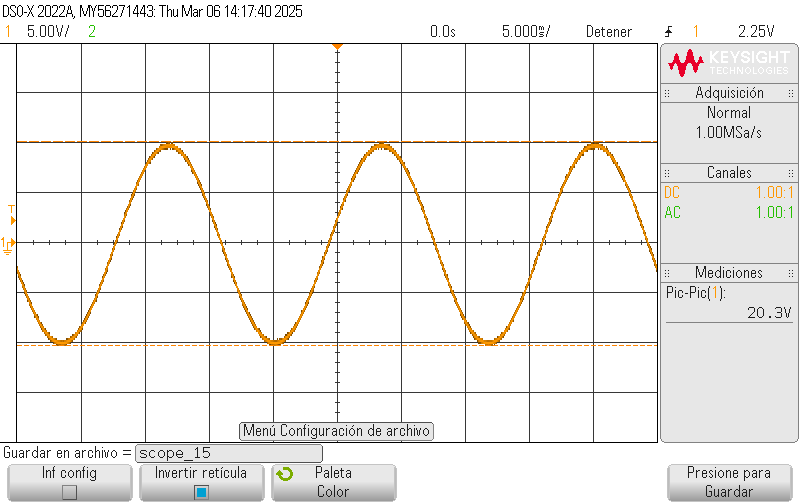
\includegraphics[width=2.8in]{SignalExperimental_01.png}
        \caption{Señal de entrada del circuito recortador sin Diodo (experimental).}
        \label{fig:SignalExperimental_01}
\end{figure}
\begin{figure}[H]
        \centering
        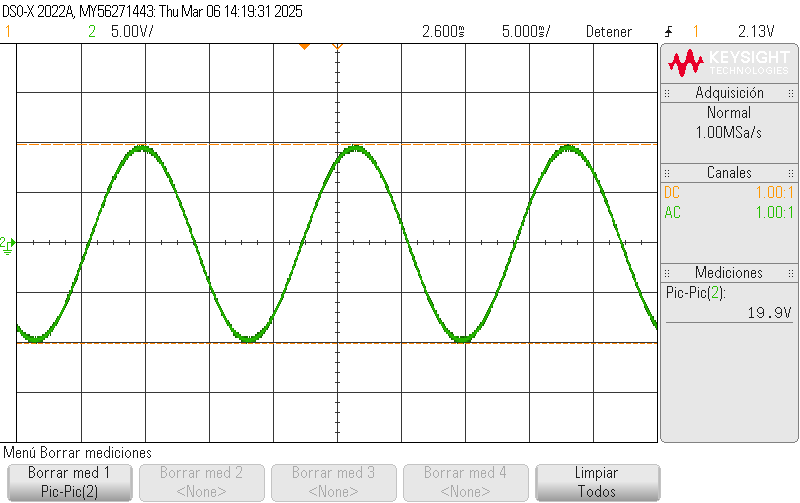
\includegraphics[width=2.8in]{SignalExperimental_02.png}
        \caption{Señal de salida del circuito recortador sin Diodo (experimental).}
        \label{fig:SignalExperimental_02}
\end{figure}

Ambas señales son muy similares, por lo que se mencionaba respecto a que los valores de la resistencia $R_2$ y $R_L$ son muy cercanos. Luego,
utilizando el circuito de la Fig. \ref{fig:recortador_conDiodo}, se obtienen las señales de entrada y salida, así como la señal de tensión presente en la resistencia $R_2$.

\begin{figure}[H]
        \centering
        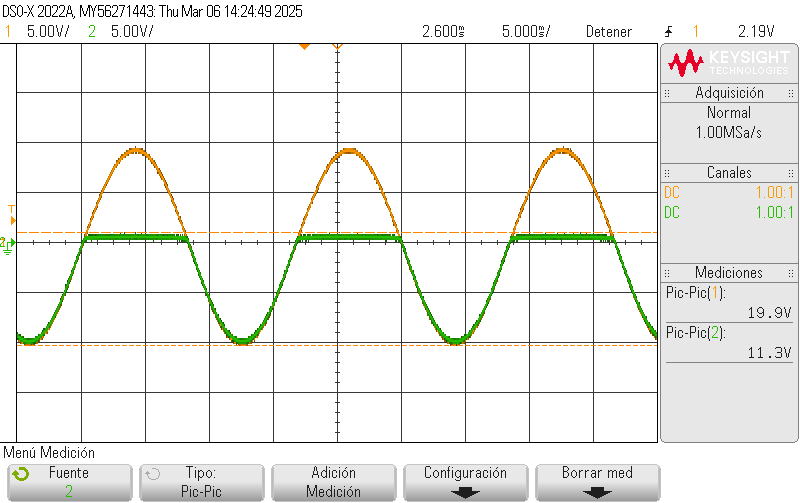
\includegraphics[width=2.8in]{SignalExperimental_03.png}
        \caption{Señales de entrada y salida del circuito recortador con Diodo (experimental).}
        \label{fig:SignalExperimental_03}
\end{figure}

\begin{figure}[H]
        \centering
        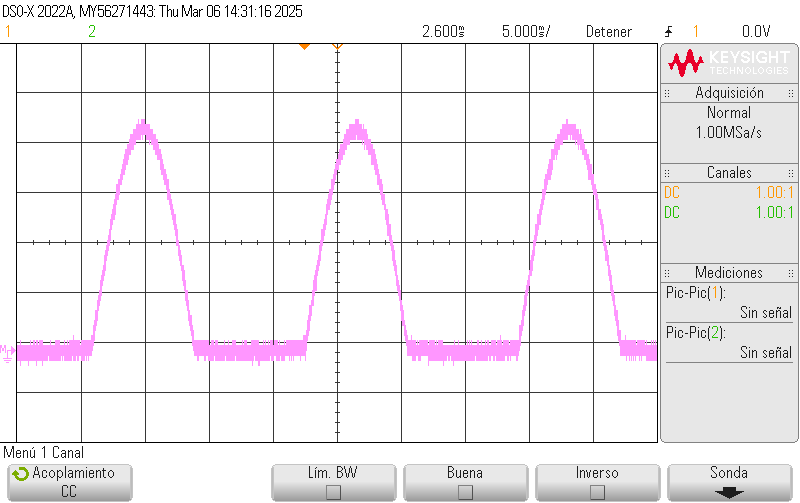
\includegraphics[width=2.8in]{SignalExperimental_04.png}
        \caption{Señal de tensión en la resistencia $R_2$ (experimental).}
        \label{fig:SignalExperimental_04}
\end{figure}

Ajustando el valor de la resistencia de carga a unos $10~\textnormal{k}\Omega$, se obtienen las siguientes señales de entrada y salida para el circuito de la Fig. \ref{fig:recortador_conDiodo}.
\begin{figure}[H]
        \centering
        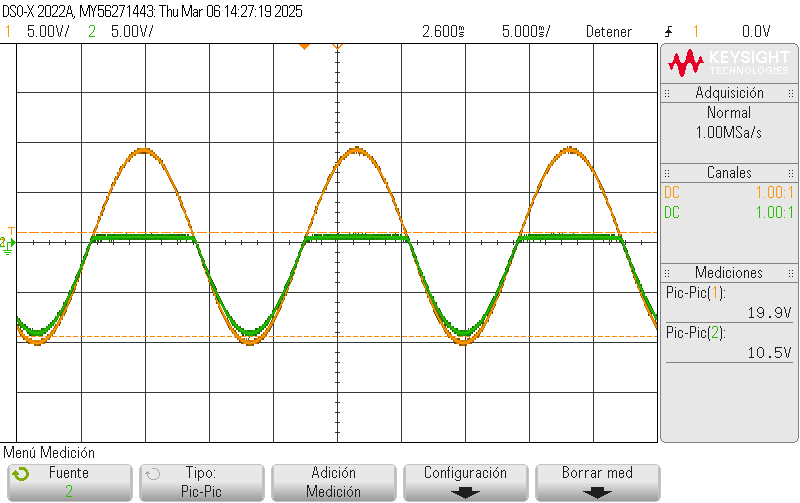
\includegraphics[width=2.8in]{SignalExperimental_05.png}
        \caption{Señales de entrada y salida del circuito recortador con Diodo, con $R_L=10~\textnormal{k}\Omega$ (experimental).}
        \label{fig:SignalExperimental_05}
\end{figure}

Como se observa, la forma de las señales son muy similares a las mostradas en la Fig. \ref{fig:SignalSimulated_04}. Ahora, se utiliza el ciruito mostrado en la Fig. \ref{fig:recortador_conAjuste}, 
con variaciones en la fuente de CD desde los $0~\textnormal{V}$ hasta los $2~\textnormal{V}$, con pasos de $500~\textnormal{mV}$.

\begin{figure}[H]
        \centering
        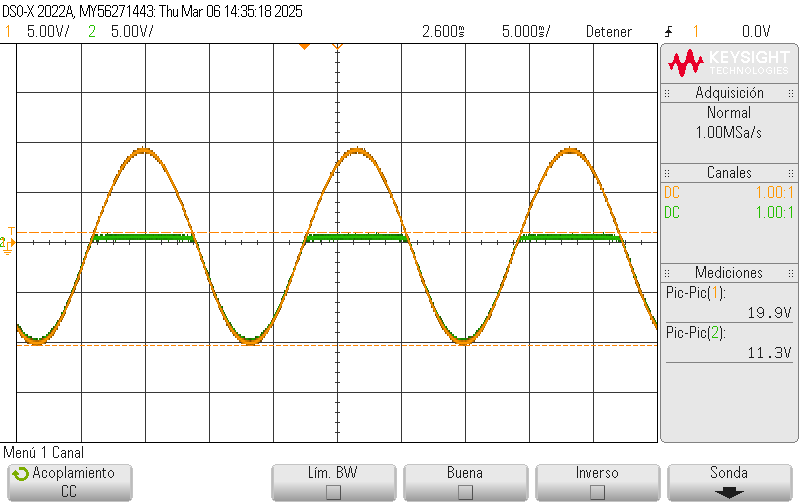
\includegraphics[width=2.8in]{SignalExperimental_06.png}
        \caption{Circuito recortador con fuente de CD en $0~\textnormal{V}$ (experimental).}
        \label{fig:SignalExperimental_06}
\end{figure}
\begin{figure}[H]
        \centering
        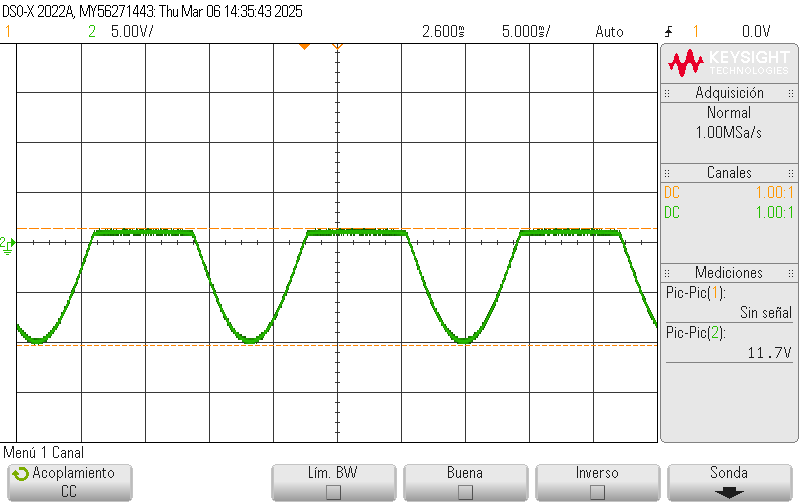
\includegraphics[width=2.8in]{SignalExperimental_07.png}
        \caption{Circuito recortador con fuente de CD en $500~\textnormal{mV}$ (experimental).}
        \label{fig:SignalExperimental_07}
\end{figure}
\begin{figure}[H]
        \centering
        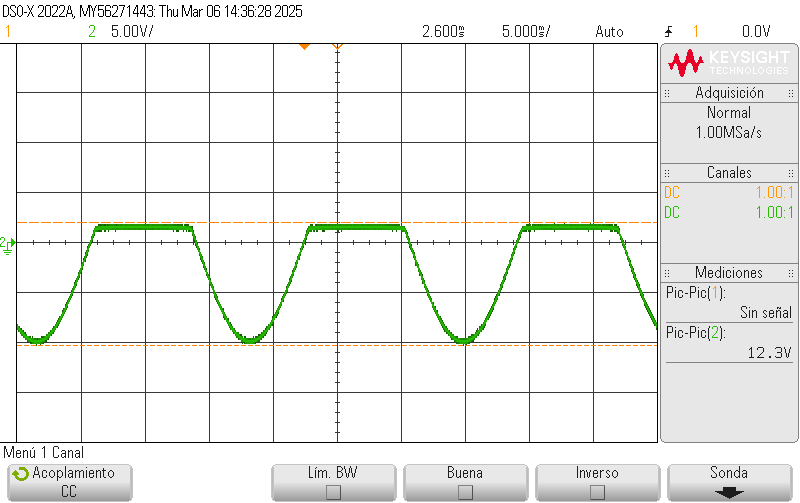
\includegraphics[width=2.8in]{SignalExperimental_08.png}
        \caption{Circuito recortador con fuente de CD en $1~\textnormal{V}$ (experimental).}
        \label{fig:SignalExperimental_08}
\end{figure}
\begin{figure}[H]
        \centering
        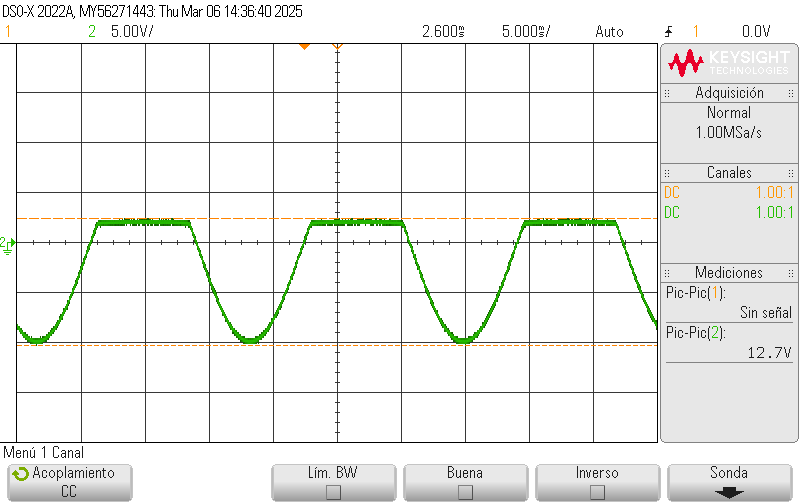
\includegraphics[width=2.8in]{SignalExperimental_09.png}
        \caption{Circuito recortador con fuente de CD en $1.5~\textnormal{V}$ (experimental).}
        \label{fig:SignalExperimental_09}
\end{figure}
\begin{figure}[H]
        \centering
        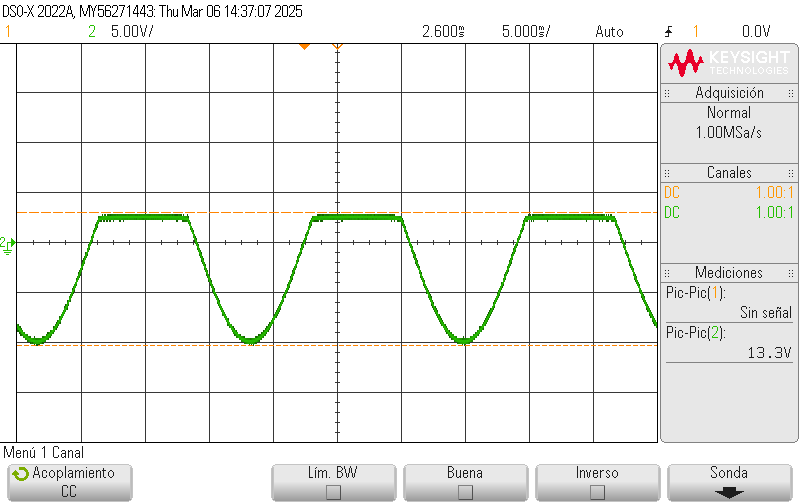
\includegraphics[width=2.8in]{SignalExperimental_10.png}
        \caption{Circuito recortador con fuente de CD en $2~\textnormal{V}$ (experimental).}
        \label{fig:SignalExperimental_10}
\end{figure}

Es posible observar como la forma de onda rectificada va aumentando su valor máximo conforme sube la tensión en la fuente de CD,
reflejando lo esperado según los datos teóricos mostrados en la sección correspondiente. 

Ahora, se repite el mismo proceso pero con la polaridad del diodo 1N914 invertida. 

\begin{figure}[H]
        \centering
        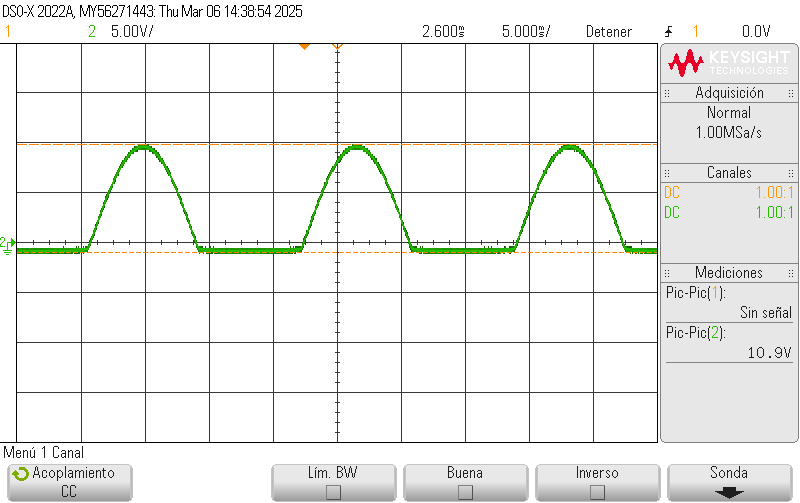
\includegraphics[width=2.8in]{SignalExperimental_11.png}
        \caption{Circuito recortador con Diodo invertido y fuente de CD en $0~\textnormal{V}$ (experimental).}
        \label{fig:SignalExperimental_11}
\end{figure}
\begin{figure}[H]
        \centering
        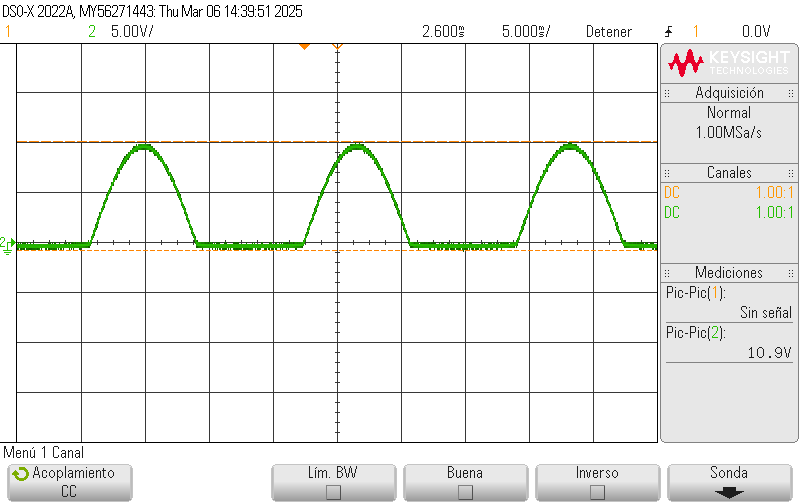
\includegraphics[width=2.8in]{SignalExperimental_12.png}
        \caption{Circuito recortador con Diodo invertido y fuente de CD en $500~\textnormal{mV}$ (experimental).}
        \label{fig:SignalExperimental_12}
\end{figure}
\begin{figure}[H]
        \centering
        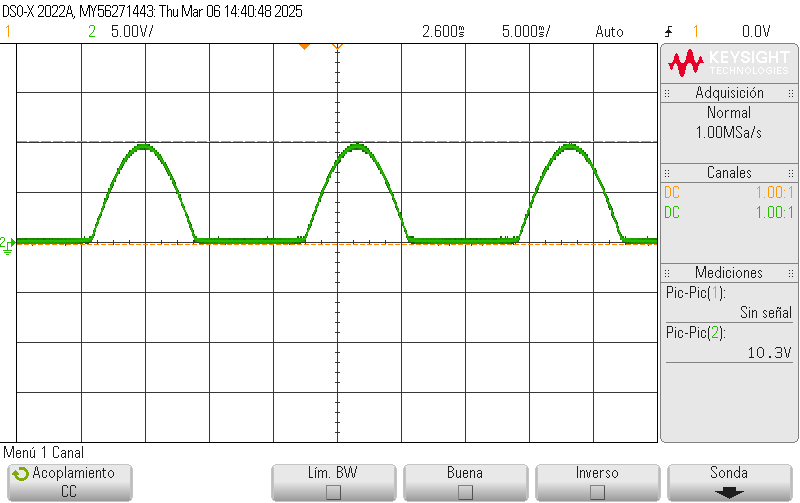
\includegraphics[width=2.8in]{SignalExperimental_13.png}
        \caption{Circuito recortador con Diodo invertido y fuente de CD en $1~\textnormal{V}$ (experimental).}
        \label{fig:SignalExperimental_13}
\end{figure}
\begin{figure}[H]
        \centering
        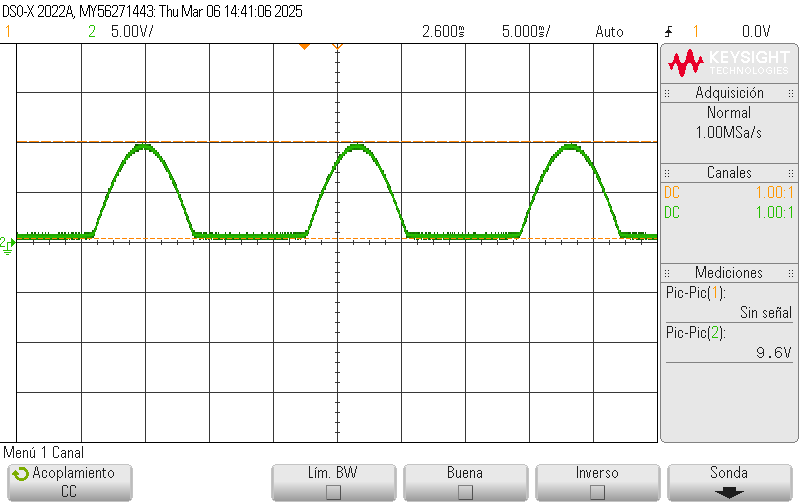
\includegraphics[width=2.8in]{SignalExperimental_14.png}
        \caption{Circuito recortador con Diodo invertido y fuente de CD en $1.5~\textnormal{V}$ (experimental).}
        \label{fig:SignalExperimental_14}
\end{figure}
\begin{figure}[H]
        \centering
        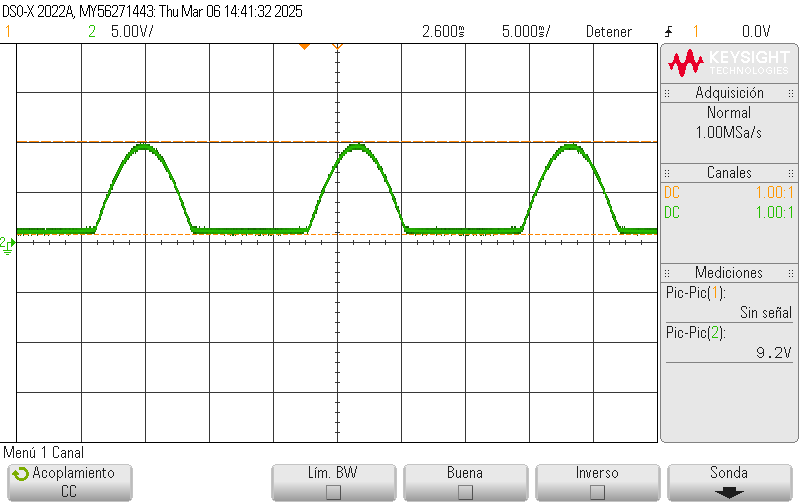
\includegraphics[width=2.8in]{SignalExperimental_15.png}
        \caption{Circuito recortador con Diodo invertido y fuente de CD en $2~\textnormal{V}$ (experimental).}
        \label{fig:SignalExperimental_15}
\end{figure}

De igual forma, se observa un ligero aumento en valor mínimo que toma la señal de salida o señal rectificada.
Luego, se modifica el circuito al invertir la polaridad de la fuente CD, haciendo que esta "brinde valores de tensión negativos".
Repitiendo el proceso de variación iterativo de la fuente desde los $0~\textnormal{V}$ hasta los $-2~\textnormal{V}$, con pasos de $500~\textnormal{mV}$.
\begin{figure}[H]
        \centering
        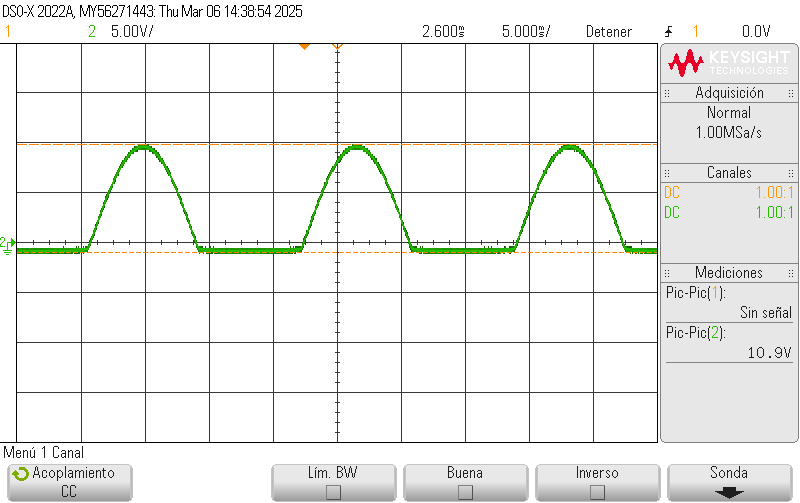
\includegraphics[width=2.8in]{SignalExperimental_11.png}
        \caption{Circuito recortador con Diodo invertido y fuente de CD en $0~\textnormal{V}$ (experimental).}
        \label{fig:SignalExperimental_16}
\end{figure}
\begin{figure}[H]
        \centering
        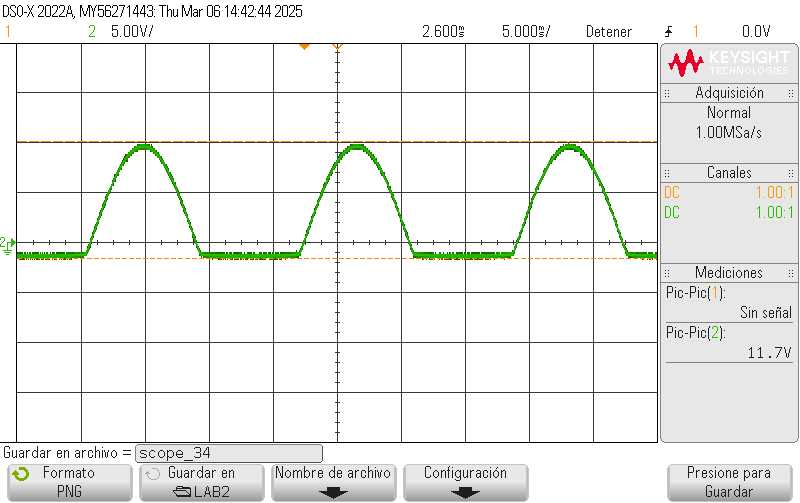
\includegraphics[width=2.8in]{SignalExperimental_16.png}
        \caption{Circuito recortador con Diodo invertido y fuente de CD en $-500~\textnormal{mV}$ (experimental).}
        \label{fig:SignalExperimental_17}
\end{figure}
\begin{figure}[H]
        \centering
        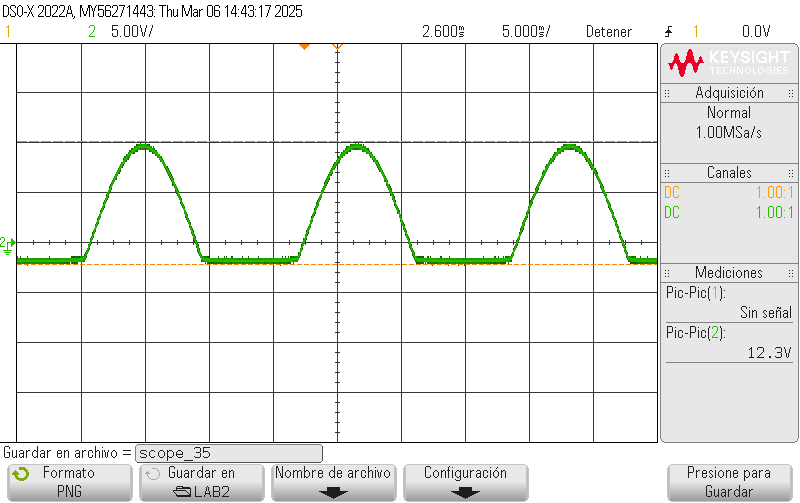
\includegraphics[width=2.8in]{SignalExperimental_17.png}
        \caption{Circuito recortador con Diodo invertido y fuente de CD en $-1~\textnormal{V}$ (experimental).}
        \label{fig:SignalExperimental_18}
\end{figure}
\begin{figure}[H]
        \centering
        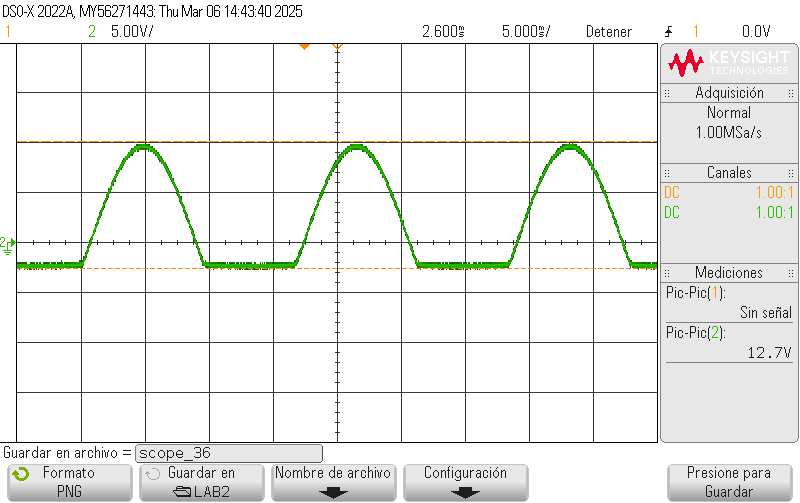
\includegraphics[width=2.8in]{SignalExperimental_18.png}
        \caption{Circuito recortador con Diodo invertido y fuente de CD en $-1.5~\textnormal{V}$ (experimental).}
        \label{fig:SignalExperimental_19}
\end{figure}
\begin{figure}[H]
        \centering
        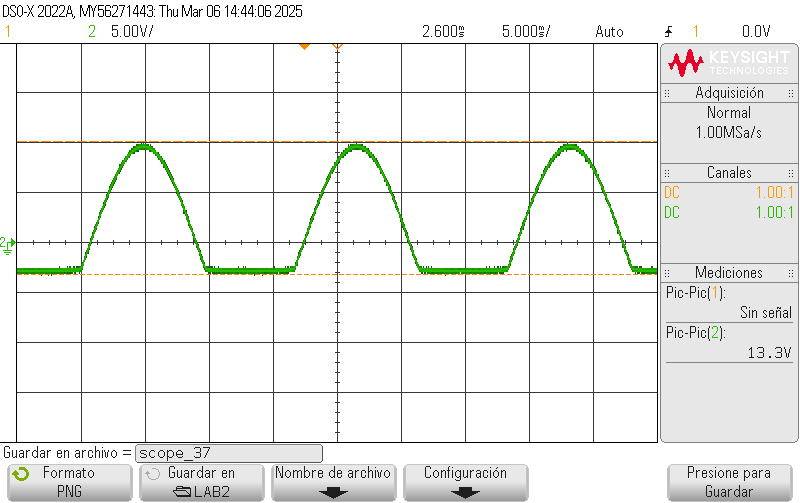
\includegraphics[width=2.8in]{SignalExperimental_19.png}
        \caption{Circuito recortador con Diodo invertido y fuente de CD en $-2~\textnormal{V}$ (experimental).}
        \label{fig:SignalExperimental_20}
\end{figure}

Aunque en este caso las señales recopiladas aparentan no tener exactamente la misma forma que las recopiladas de forma simulada,
esto se debe a un tema de escala y persepctiva, pues las ondas sí disminuyen su valor mínimo en el pico negativo de cada periodo.



\subsection{Análisis de Resultados}
Los resultados obtenidos en el laboratorio fueron satisfactorios, lo que permite considerar la experiencia como provechosa. 
Entre los aspectos más destacados se encuentra el mayor entendimiento de la estructura general de cada uno de los circuitos utilizados, 
resultado de la interacción directa con componentes y dispositivos físicos. Esto resalta la importancia de prestar atención a las conexiones y a los 
métodos de medición para garantizar la recolección de datos de manera correcta y precisa.

Los datos y gráficas obtenidos reflejaron el comportamiento esperado y previamente estudiado en el entorno de simulación. 
Sin embargo, se observaron algunas variaciones en ciertas magnitudes del circuito (al momento de alterar ciertas conexiones por razones varias), 
lo que requirió ajustes en los parámetros de medición de los equipos. 
Para mejorar la interpretación de los resultados, es necesario considerar posibles alteraciones en las señales debidas a escalas de 
representación o interferencias de ruido.

\section{Conclusiones}
Se puede apreciar que las ondas de salida obtenidas durante el experimento siguieron la forma que se esperaba. A pesar de pequeñas diferencias
en cuanto a las amplitudes esperadas, el comportamiento general de la onda fue el calculado, por lo que el objetivo del experimento de construir circuitos recortadores
para entender el comportamiento de distintas ondas de salida fue cumplido exitosamente.

\appendices

\section{}
\vspace{-1.2cm}
\begin{IEEEbiographynophoto}{Matías A. Camacho Abarca}
        Estudiante del Instituto Tecnológico de Costa Rica en la carrerra de ingeniería en electrónica desde
        2023. Beneficiario de beca de excelencia académica por el Instituto Tecnológico de
        Costa Rica desde 2023. Como estudiante, sus
        intereses incluyen investigación y desarrollo.
        Correo electrónico: jeacamacho@estudiantec.cr
\end{IEEEbiographynophoto}
\vspace{-1.2cm}
\begin{IEEEbiographynophoto}{Juan P. Elizondo Espinoza}
        Oriundo de Pérez Zeledón. Realizó sus estudios de secundaria en el SNCCCR, sede UNA Región Brunca, y actualmente cursa la carrera de Ingeniería Electrónica en el Instituto Tecnológico de Costa Rica (TEC). 
        
        Anteriormente, fue estudiante de la Universidad de Costa Rica (UCR) durante el año 2022 y participó en programas de estudio en matemática en la Universidad Nacional (UNA) durante los años 2020 y 2021. 
        
        Cuenta con preparación y/o experiencia en áreas como:
        \begin{itemize}
            \item Arquitectura básica de redes, certificado por CISCO CCNA V7 (ITN), (2021).
            \item Principios de ciberseguridad, certificado por CISCO Systems, (2022).
            \item Programa de tutorías estudiantiles, Tecnológico de Costa Rica, (2024).
        \end{itemize}
        
        Correo: juelizondo@estudiantec.cr
\end{IEEEbiographynophoto}

\bibliographystyle{IEEEtran}
\bibliography{literatura}

\end{document}